\documentclass[11pt]{article}
\usepackage{times}
\usepackage{ifthen}
\usepackage[dvips]{graphics}
\usepackage[dvips]{color}
\usepackage{epsfig}
%\usepackage{subfigure}
\usepackage[dvips, colorlinks, bookmarks, pdfpagemode=UseOutlines,
linkcolor=blue, pagecolor=blue, urlcolor=blue, letterpaper]{hyperref}
\begin{document}
% File giving definitions of commands and environments.
% Because of a latex bug with counters, this has to be included
% using \input not \include.

%--------------------------------------------------------------------------
% For the set of reals and integers
\newcommand{\rr}{\set{Reals}}
\newcommand{\ii}{\set{Integers}}
\newcommand{\cc}{\set{Complex}}
\newcommand{\nn}{\set{Naturals}}

%--------------------------------------------------------------------------
% For figure captions.
% Puts them in sanserif font, indented on both sides.
%   arg: The caption.
\newcommand{\figcaption}[1]{\textsf{\begin{center}\begin{minipage}{5in}
\caption{#1}
\end{minipage}\end{center}}}

%--------------------------------------------------------------------------
% For terms being defined.
% Puts them in bold face and creates an index entry.
%   arg: The term being defined.
% NOTE: To get boldface in the index, do |textbf after #1.
% But this breaks hyperlinks.
\newcommand{\defn}[1]{\textbf{#1}\index{#1}}

%--------------------------------------------------------------------------
% For terms being indexed.
% Puts them in standard font face and creates an index entry.
%   arg: The term being defined.
\newcommand{\pointer}[1]{#1\index{#1}}

%--------------------------------------------------------------------------
% For bold terms to be index, but defined elsewhere
% Puts them in bold face and creates an index entry.
%   arg: The term being defined.
\newcommand{\strong}[1]{\textbf{#1}\index{#1}}

%--------------------------------------------------------------------------
% For terms to be index, but defined elsewhere
% Puts them in normal face and creates an index entry.
%   arg: The term being defined.
\newcommand{\idx}[1]{#1\index{#1}}

%--------------------------------------------------------------------------
% For set names.
% Puts them in italics. In math mode, yields decent spacing.
%   arg: The name of the set.
\newcommand{\set}[1]{\mbox{\textit{#1}}}

%--------------------------------------------------------------------------
% For real part.
%   arg: The argument of the real part.
\newcommand{\re}[1]{\mbox{\textit{Re}}\{#1\}}

%--------------------------------------------------------------------------
% For imaginary part.
%   arg: The argument of the imaginary part.
\newcommand{\im}[1]{\mbox{\textit{Im}}\{#1\}}

%--------------------------------------------------------------------------
% For matlab commands
%   arg: The name of the command
\newcommand{\matlab}[1]{\texttt{#1}\index{#1 command in Matlab}\index{Matlab!#1}}
\newcommand{\simulink}[1]{\texttt{#1}\index{#1 in Simulink}\index{Simulink!#1}}
\newcommand{\matlabInCaption}[1]{\texttt{#1}}

%--------------------------------------------------------------------------
% For "Probing Further" sidebars.
% Puts them in a floating frame.  It is up to you to ensure that the
% frame fits on one page.
%   arg: the title.
\newenvironment{further}[1]{
\begin{table}[btp]
\centering
\begin{tabular}{|p{5in}|}
\hline
\cr
\begin{minipage} {5in}
\parskip        0.1in
\parindent      0.0in
\subsection* {Probing further: #1}
\addcontentsline{toc}{subsection}{Probing further: #1}
} {
\end{minipage}\cr
\cr
\hline
\end{tabular}
\end{table}
}

%--------------------------------------------------------------------------
% For "Basics" sidebars.
% Puts them in a floating frame.  It is up to you to ensure that the
% frame fits on one page.
%   arg: the title.
\newenvironment{basics}[1]{
\begin{table}[btp]
\centering
\begin{tabular}{|p{5in}|}
\hline
\cr
\begin{minipage} {5in}
\parskip        0.1in
\parindent      0.0in
\subsection* {Basics: #1}
\addcontentsline{toc}{subsection}{Basics: #1}
} {
\end{minipage}\cr
\cr
\hline
\end{tabular}
\end{table}
}

%--------------------------------------------------------------------------
% For "Tips and Tricks" sidebars.
% Puts them in a floating frame.  It is up to you to ensure that the
% frame fits on one page.
%   arg: the title.
\newenvironment{tricks}[1]{
\begin{table}[btp]
\centering
\begin{tabular}{|p{5in}|}
\hline
\cr
\begin{minipage} {5in}
\parskip        0.1in
\parindent      0.0in
\subsection* {Tips and Tricks: #1}
\addcontentsline{toc}{subsection}{Tips and Tricks: #1}
} {
\end{minipage}\cr
\cr
\hline
\end{tabular}
\end{table}
}

%--------------------------------------------------------------------------
% For text that is boxed for emphasis.
\newenvironment{boxed}{
\begin{center}
\begin{tabular}{|p{5in}|}
\hline
\cr
\begin{minipage} {5in}
\parskip        0.1in
\parindent      0.0in
} {
\end{minipage}\cr
\cr
\hline
\end{tabular}
\end{center}
}

%--------------------------------------------------------------------------
% For examples
% NOTE: Because of this line, this has to be included using \input
% not \include.
\newcounter{example}
\newenvironment{example}{
\refstepcounter{example}
\begin{quote}
\textbf{Example \arabic{chapter}.\arabic{example}:}
} {
\end{quote}
}
\renewcommand \theexample {\thechapter.\arabic{example}}


\title{A 2D Algorithm for SoftWalls}

\author{J. Adam Cataldo, Edward A. Lee, Xiaojun Liu, Ashwin Ganesan,\\
and Stephen Neuendorffer\\ 
\{acataldo, eal, liuxj, ganesan, neuendor\}@eecs.berkeley.edu\\
Electrical Engineering \& Computer Science\\ 
University of California, Berkeley\\ 
\\}

\date{19 July 2002}
\maketitle

%-----------------------------------------------------------------------------
%-----------------------------------------------------------------------------

\section{Introduction}

This document gives an outline of a general 2D softwalls approach.

%-----------------------------------------------------------------------------
%-----------------------------------------------------------------------------


\section{Control with Bias}

%-----------------------------------------------------------------------------

Suppose the aircraft is travelling at a constant speed $s$.  Let
$\theta$ denote the aircraft's heading angle, and let
$\dot{\theta_{p}}$ be the pilot's control input, i.e. the desired rate
of change in heading angle.  With speed $s$ the aircraft has a
minimum-safe turning radius $r_{min}$.  The paths an aircraft travels
as it banks right or left with radius $r_{min}$ are in figure \ref{paths}.

\begin{figure}[btp]
\centering
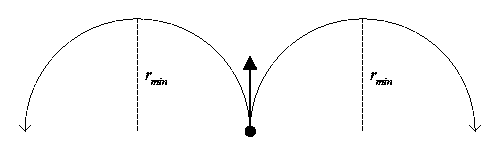
\includegraphics[width=5in]{aircraftpaths.eps}
\figcaption{The dot represents the aircraft, which is moving along the
center path.  The circle paths represtent turns at the minimum turning radius.
\label{paths}}
\end{figure}

Now suppose we wish to prevent the aircraft from entering a no-fly
zone.  As the aircraft approaches the no-fly zone boundary, one of the
minimum-turning-radius paths from figure \ref{paths} will interesect
with the boundary.  As long as the other path has not yet
interestected the boundary, the aircraft can still avoid crossing the
boundary by moving along this path.  At the instant the second path
intersects the boundary, forcing the aircraft to fly along the second
path will prevent the aircraft from crossing the boundary.  This
situation is depicted in figure \ref{crossing}.

\begin{figure}[btp]
\centering
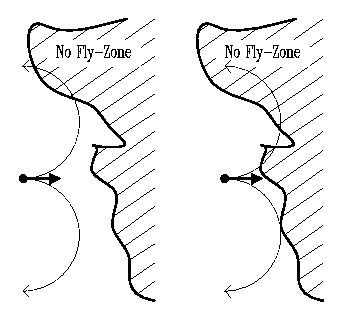
\includegraphics[width=5in]{boundarycross.eps}
\figcaption{On the left picture, the aircraft still has one free path.  On the
right picture, the aircraft must move right at the minimum turning
radius to avoid crossing the boundary.
\label{crossing}}
\end{figure}

We can think of this algorithm as applying a bias to the pilot's
desired rate of change in heading.  Let the actual rate of change in
aircraft heading angle be $\dot{\theta}$, and let $\theta_{s}$, be the
control signal generated by the SoftWalls algorithm.  Given the
pilot's desired rate of change in heading, $\dot{\theta_{p}}$, we
calculate $\dot{\theta}$ from
\begin{equation}
\dot{\theta} = limit_{[-s/r_{min}, s/r_{min}]}(\dot{\theta_{p}} -
\dot{\theta_{s}}),
\label{control}
\end{equation}
where
\[
\set{limit}_{[a,b]}(u) = \left \{
\begin{array}{ll}
b&\mbox{ if } u > b,\\
a&\mbox{ if } u < a,\\
u&\mbox{ otherwise. }
\end{array}
\right .
\]
By limiting $\dot{\theta}$ to the range $[-s/r_{min}, s/r_{min}]$, we
ensure that no safe turn is made.

Assuming $\dot{\theta_{p}}$ is limited to $[-\dot{\theta_{M}},
\dot{\theta_{M}}]$, which corresponds to the limits of the flight
yoke, we can choose $\dot{\theta_{s}} = \dot{\theta_{M}} + s/r_{min}$
to force the aircraft to turn right at the maximum turning radius,
irrespective of pilot input.  This works because this value of
$\dot{\theta_{s}}$ makes $\dot{\theta}$ in equation \ref{control}
equal to $s/r_{min}$ for any $\dot{\theta_{p}} \in [-\dot{\theta_{M}},
\dot{\theta_{M}}]$.  Similarly $\dot{\theta_{s}} = -\dot{\theta_{M}} -
s/r_{min}$ will force the aircraft to turn left.  If the right path is
the second path to interesect the boundary, the control signal
$\dot{\theta_{s}} = \dot{\theta_{M}} + s/r_{min}$ will steer the
aircraft right, and if the left path is the second to interestect the
boundrary, the control signal $\dot{\theta_{s}} = -\dot{\theta_{M}} -
s/r_{min}$ will steer the aircraft left.  By applying the appropriate
$\theta_{s}$ to the input, the SoftWalls algorithm (the
path/boundary-interestection algorithm) can garauntee the plane to
never crosses the boundary.  This is a step bias, because the bias is
either present or absent.

\section{Smooth Bias}

The method in the previous section takes all control away from the
pilot when the bias is applied, and returns all control when the bias
is turned off.  This can be dangerous because a pilot may not be ready
to take the aircraft over again when the bias is turned off.  We would
like to increase and decrease the bias smoothly to prevent this
situation.

To apply a smooth bias, we first draw a circle of radius $r_{o}$
around each path of radius $r_{min}$ in figure \ref{paths}, as in
figure \ref{circles}.  We choose $r_{min} < r_{o} < 2r_{min}$, so that
the larger circles do not encircle the centers of the opposing
circles.  We call the circular path that a plane would take to go
right at the minimum turning radius the \textit{r-path} and the center
of this circle the \textit{r-circle}.  We call the circle of radius
$r_{o}$ centered at r-center the \textit{r-extension}, because it will
be used to extend the region of SoftWalls bias for smooth control.
Similarly the \textit{l-path} is the circular path that a plane would
take to go left at the minimum turning radius, which is centered at
the \textit{l-center} and surrounded by the \textit{l-extension}.


\begin{figure}[btp]
\centering
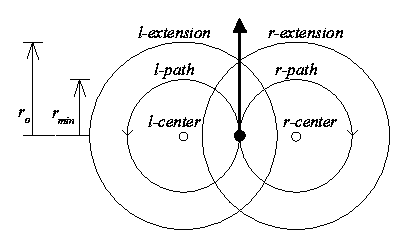
\includegraphics[width=5in]{circles.eps}
\figcaption{The black dot represents the aircraft, and the dark arrow
represents its current path.  The r-path represents a right turn at
the minimum turning radius and the l-path represents a left turn at
teh minimum turning radius.
\label{circles}}
\end{figure}


When none of the two extension circles intersect the no-fly-zone
boundary, the SoftWalls bias is zero.  At any instant, we are
interested in two points on the boundary.  The one closest to r-center
has distance $d_{r}$ from r-center, and the one closest to l-center
has distance $d_{l}$.  When one of the extension circles, say
l-extension, crosses the boundary, the bias remains zeros until the
second circle, r-extension, intersects the boundary.  At that point
the bias increases linearly as $d_{r}$ decreases up to the point
where the r-path intersects the boundary, and the maximum bias is
applied:
\[
\dot{\theta_{s}} = \frac{d_{r} - r_{min}}{r_{o} - r_{min}}
(\dot{\theta_{M}} + s/r_{min})
\]

When the l-extension leaves the no-fly zone, we should decrease the
bias linearly as $d_{l}$ increases, until there is zero bias applied:
\[
\dot{\theta_{s}} = \max{ \{(\frac{d_{r} - r_{min}}{r_{o} - r_{min}} +
\frac{r_{o} - d_{l}}{r_{o} - r_{min}}) (\dot{\theta_{M}} + s/r_{min}),
0 \}}
\]
Then at the point where the resistant pilot's aricraft is parallel to
the wall at distance $2r_{min}$, zero bias is applied, and an escape
path is available.

\end{document}








